\section{Definisi Cloud Computing}
\tab Cloud Computing yang dalam pengertian bahasa Indonesia diterjemahkan menjadi komputasi awan, beberapa tahun terakhir ini telah menjadi "Hot word" di dunia teknologi informasi (TI). Seluruh nama besar seperti IBM, Microsoft, Google, dan Apple, saat ini sedang terlibat dalam peperangan untuk menjadi penguasa terbesar terhadap awan ini. Tentu saja masing-masing mengeluarkan jurusnya sendiri-sendiri. IBM di paruh akhir tahun 2009 kemarin telah meluncurkan LotusLive, layanan kolaborasi berbasis cloud. Microsoft, yang sekarang di perkuat oleh Ray Ozzie sebagai Chief Software Architect pengganti Bill Gates, menggadang Windows Azure, sistem operasi berbasis cloud yang akan menjadi masa depan Windows OS.\\
\tab Apple mengambil sisi lain, telah menyediakan layanan Mobile Me yang memungkinkan pengguna produk Mac, untuk melakukan sinkronisasi data ke Dalam cloud. Sementara google "raksasa yang lahir di era internet sudah sejak lama memberikan suatu layanan yang dikenal dengan nama "Google Docs". Dengan layanan ini memungkinkan user dapat membuat dokumen atau dapat bekerja kerja dengan spread sheet secara online tanpa perlu menginstall software di PC atau Notebook. Bahkan google juga meluncurkan system operasi cloud-nya, yang sistem operasi alternative dari system operasi yang sudah ada, yang mungkin juga menjadi "ancaman" serius bagi penyedia sistem operasi. Sebelum kita membahas lebih jauh mengenai Cloud Computing,terlebih dahulu pada bab ini kita akan membahas definisi dari CLOUD COMPUTING. Untuk itu mari kita lihat beberapa definisi dari Cloud Computing, agar kita dapat mengenal dan mengerti dengan jelas apa itu Cloud Computing? kemana tujuanya? dan apa resikonya? dan bagaimana organisasi IT atau praktisi IT mempersiapkan ini? inilah pertanyaan yang setidaknya akan hadir bagi beberapa praktisi ataupun peminat IT dibawah ini ada beberapa definisi Cloud Computing yang dapat membantu kita untuk mengenal apa itu Cloud Computing:
\begin{itemize}
\item Cloud Computing adalah gabungan pemanfaatan teknologi komputer ('komputasi') dan pengembangan berbasis Internet ('awan'). Awan (cloud) adalah metefora dari internet, sebagaimana awan yang sering digambarkan di diagram jaringan komputer, awan (cloud) dalam Cloud Computing juga merupakan abstraksi dari infrastruktur kompleks yang disembunyikannya. Internet Cloud adalah suatu model komputasi di mana kapabilitas terkait teknologi informasi disajikan sebagai suatu layanan, sehingga pengguna dapat mengaksesnya lewat Internet.
\item Cloud Computing adalah suatu konsep umum yang mencakup SaaS(software as a service), Web 2.0, dan tren teknologi terbaru lain yang dikenal luas, dengan tema umum berupa ketergantungan terhadap Internet untuk memberikan kebutuhan komputasi pengguna.
\item Cloud computing adalah istilah untuk kegiatan menyelesaikan suatu proses atau perhitungan melalui internet dengan memanfaatkan sumber daya yang dimiliki oleh suatu kumpulan komputer yang saling terhubung di suatu tempat.
\item Cloud computing adalah teknologi yang menggunakan internet dan server pusat yang jauh untuk menjaga/mengelola data dan aplikasi.
\item Cloud Computing secara sederhana dapat didefinisikan adalah "layanan teknologi informasi yang bisa dimanfaatkan atau diakses oleh pelanggannya melalui jaringan internet". Kata-kata "Cloud" sendiri merujuk kepada simbol awan yang di dunia TI digunakan untuk menggambarkan jaringan internet (internet cloud).
\item Cloud Computing bisa diartikan sebagai suatu model yang memungkinkan jaringan dapat diakses dengan mudah sesuai kebutuhan di berbagai lokasi.dimana model ini memungkinkan untuk mengumpulkan sumber daya komputasi seperti network, server, storage, aplikasi dan services dalam satu wadah.
\end{itemize}
\tab Menurut sebuah makalah tahun 2008 yang dipublikasikan IEEE Internet Computing Cloud Computing merupakan suatu paradigma dimana suatu informasi secara permanen tersimpan di server (di Internet) dan tersimpan secara sementara di computer pengguna (client) termasuk di dalamnya adalah desktop, computer tablet, notebook, sensor-sensor dan lain lain. Melihat perkembangan saat ini, maka yang dibutuhkan oleh organisasi IT ataupun Praktisi IT adalah memberikan berbagai macamlayanan terdistribusi dan pararel secara remote dan dapat berjalan di berbagai device, dan teknologinya dapat dilihat dari berbagai teknologi yang digunakan dari proses informasi yang diaplikaikan secara outsourcing sampai dengan penggunaan eksternal data center. Cloud Computing merupakan model yang dapat mendukung layanan "Everything as a sevice" (XaaS). Sehingga dapat mengintegrasikan virtualized physical sources, virtualized infrastructure.
\tab Cloud computing atau komputasi awan merupakan tren baru di bidang komputasi terdistribusi dimana berbagai pihak dapat mengembangkan aplikasi dan layanan berbasis SOA (Service Oriented Architecture) di jaringan internet. Definisi dan batasan dari Cloud Computing sendiri masih mencari bentuk dan standarnya. Dimana pasarlah yang akan menentukan model mana yang akan bertahan dan model mana yang akan berakhir. Namun semua sepakat bahwa Cloud Computing akan menjadi masa depan dari dunia komputasi. Bahkan lembaga riset bergengsi Gartner Group juga telah menyatakan bahwa Cloud Computing adalah wacana yang tidak boleh dilewatkan oleh seluruh organisasi IT ataupun praktisi IT yang berkepentingan di dunia IT, mulai saat ini dan dalam beberapa waktu mendatang. Ini disebabkan karena Cloud Computing adalah sebuah mekanisme yang memungkinkan kita "menyewa" sumber daya teknologi informasi (software, processing power, storage, dan lainnya) melalui internet dan memanfaatkan sesuai kebutuhan kita dan membayar sesuai dengan yang digunakan oleh kita saja.
\tab Dengan konsep ini, maka semakin banyak orang yang bisa memiliki akses dan memanfaatkan sumber daya tersebut, karena tidak harus melakukan investasi besar-besaran. Apalagi dalam kondisi ekonomi seperti sekarang, setiap organisasi akan berpikir panjang untuk mengeluarkan investasi tambahan di sisi IT. Terlebih hanya untuk mendapatkan layanan-layanan yang mungkin hanya dibutuhkan sewaktu-waktu saja. Sebagaimana telah dijelaskan pada defenisi di atas bahwa Cloud Computing adalah layanan teknologi informasi yang di manfaatkan melalui jaringan Internet, namun tidak semua layanan yang ada di Internet dapat dikategorikan sebagai layanan Cloud Computing. Ada pun beberapa syarat yang harus dipenuhi agar layanan yang ada di Internet dikatakan sebagai layanan Cloud Computing :
\begin{enumerate}
\item Layanan bersifat "On Demand", pengguna dapat berlangganan hanya yang dia butuhkan saja, dan membayar hanya untuk yang mereka gunakan saja. Misalkan sebuah sebuah internet service provider menyediakan 5 macam pilihan atau paket-paket internet dan user hanya mengambil 1 paket internet maka user hanya membayar paket yang diambil saja.
\item Layanan bersifat elastis/scalable, di mana pengguna bisa menambah atau mengurangi jenis dan kapasitas layanan yang dia inginkan kapan saja dan sistem selalu bisa mengakomodasi perubahan tersebut. Misalkan user berlangganan internet pada yang bandwidthnya 512 Kb/s lalu ingin menambahkan kecepatannya menjadi 1Mb/s kemudian user menelpon costumer service meminta untuk penambahan bandwitch lalu customer service merespon dengan mengubah bandwidth menjadi 1Mb/s.
\item Layanan sepenuhnya dikelola oleh penyedia/provider, yang dibutuhkan oleh pengguna hanyalah komputer personal/notebook ditambah koneksi internet.
\item Sumber Daya Terkelompok (Resource pooling) \\Penyedia layanan Cloud Computing memberikan layanan melalui sumber daya yang dikelompokkan di satu atau berbagai lokasi data center yang terdiri dari sejumlah server dengan mekanisme multi-tenant. Mekanisme multi-tenant ini memungkinkan sejumlah sumber daya komputasi digunakan secara bersama-sama oleh sejumlah user, dimana sumber daya tersebut baik yang berbetuk fisik atau virtual, dapat dialokasikan secara dinamis untuk kebutuhan pengguna / pelanggan sesuai permintaan. Dengan demikian pelanggan tidak perlu tahu bagaimana dan darimana permintaan akan sumber daya komputasinya terpenuhi oleh penyedia layanan yang ada di Cloud Computing. Yang penting setiap permintaan dapat dipenuhi. Sumber daya komputasi ini meliputi media penyimpanan, memory, processor, pita jaringan dan mesin virtual.
\item Akses Pita Lebar \\Layanan yang terhubung melalui jaringan pita lebar, terutama dapat diakses secara memadai memalui jaringan internet. Baik menggunakan thin client, thick client, ataupun media lain seperti smartphone.
\item Layanan yang terukur. (Measured Service) \\Sumber daya cloud yang tersedia harus dapat diatur dan dioptimasi penggunaannya, dengan suatu sistem pengukuran yang dapat mengukur penggunaan dari setiap sumber
daya komputasi yang digunakan (penyimpanan, memory, processor, lebar pita, aktivitas user, dan lainnya). Dengan demikian, jumlah sumber daya yang digunakan dapat secara transparan diukur yang akan menjadi dasar bagi user untuk membayar biaya penggunaan layanan.
\end{enumerate}
\tab Selain itu karakterisik dari Cloud Computing adalah sangat cepat di deploy, instant untuk implementasi. Dalam hal ini :
\begin{itemize}
\item Biaya start up teknologi ini (Cloud Computing) mungkin akan sangat murah ataupun tidak ada, dan juga tidak ada investasi kapital.
\item Biaya dari service dan pemakaian akan berdasarkan komitmen yang tidak fix.
\item Pelayanan ini (Cloud Computing) dapat dengan mudah di upgrade atau downgrade dengan cepat tanpa adanya "penalty".
\item Pelayanan akan menggunakan metode multi-tenant (banyak customer dalam 1 platform).
\item Kemampuan untukmeng-customize pelayanan akan menjadi terbatas.
\end{itemize}
\tab Dilihat dari jenis layanan tersendiri, Cloud Computing, terbagi dalam 3 jenis layanan (secara umum), yaitu Software as a Service (SaaS), Platform as a Service (PaaS) dan Infrastructure as a Service (IaaS). Namun secara spesifik layanan Cloud Computing lebih dari 3 jenis layanan. Yaitu : SaaS (Service as a Service),Utility Computing, Web Service, MSP (Management Service Provider), E-Commerce, Intergrated Network. Pembahasan mengenai jenis-jenis layanan ini akan di bahas lebih detail pada bab 3 (pembahasan di dalam buku ini). Sementara dari sifat jangkauan layanan, Cloud Computing terbagi menjadi 4 jenis layanan yaitu Public Cloud, Private Cloud, Communuity Cloud dan Hybrid Cloud.
\begin{enumerate}
\item Public Cloud \\Jenis cloud ini diperuntukkan untuk umum oleh penyedia layanannya.
\item Private Cloud \\Merupakan infrastruktur layanan cloud, yang dioperasikan hanya untuk sebuah
organisasi tertentu. Infrastruktur cloud itu bisa saja dikelola oleh sebuah organisasi itu atau oleh pihak ketiga. Lokasinya pun bisa on-site ataupun off-site. Biasanya organisasi dengan skala besar saja yang mampu memiliki/mengelola private cloud ini.
\item Community cloud \\Dalam model ini, sebuah infrastruktur cloud digunakan bersama-sama oleh beberapa
organisasi yang memiliki kesamaan kepentingan, misalnya dari sisi misinya, atau tingkat keamanan yang dibutuhkan, dan lainnya.
\item Hybrid Cloud \\Untuk jenis ini, infrastruktur cloud yang tersedia merupakan komposisi dari dua atau lebih infrastruktur cloud (private, community, atau public). meskipun secara entitas mereka tetap berdiri sendiri, tapi dihubungkan oleh suatu teknologi / mekanisme yang memungkinkan portabilitas data dan aplikasi antar cloud itu. Misalnya, mekanisme load balancing yang antar cloud, sehingga alokasi sumberdaya bisa dipertahankan pada level yang optimal. \\Berikut adalah beberapa gambar konsep atau ilustrasi dari Cloud Computing.
\end{enumerate}
\begin{center}
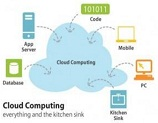
\includegraphics[scale=1]{saatu.jpg} \\
\textbf{Gambar 1.1} Ilustrasi Cloud Computing
\end{center}
\begin{center}
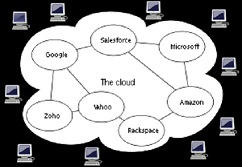
\includegraphics[scale=1]{sdua.jpg} \\
\textbf{Gambar 1.2} Diagram Konsep Cloud Computing
\end{center}
\tab yang menjadi pertanyaan, Apa bedanya dengan pemakaian komputer biasa selama ini? Pada pemakaian komputer biasa, diperlukan sistem operasi dan program aplikasi. Sistem operasi sangat menentukan program aplikasi. Kalau pemakai memilih sistem operasi MS Windows misalnya, maka aplikasinya pun harus berbasis Windows. Demikian juga kalau sistemnya berbasis DOS, Linux, Mac, dan sebagainya. Padahal memilih sistem operasi sendiri sering membuat user pusing, mau yang gratisan, atau yang berbayar? Program aplikasi harus dipasang di komputer sesudah sistem operasi terpasang. \\Untuk aplikasi berbasis DOS, relatif gampang, karena tidak perlu diinstal. Asal dikopi ke komputer, sudah siap dijalankan. Aplikasi ini sering disebut dengan stand alone software, karena tidak dapat dijalankan bersamaan dengan program lain. Keuntungannya, bila akan dijalankan di komputer lain, tinggal disalin saja, selesai. Tapi kalau sistemnya berbasis grafis dan multitasking (seperti MS Windows), program harus diinstal dulu. Kalau komputer lain diinginkan untuk menjalankan aplikasi tersebut, harus diisi dengan proses instal lagi, tidak bisa hanya dengan disalin seperti pada sistem DOS. Program seperti ini disebut dengan desktop application. Keunggulannya, dapat berjalan bersamaan dengan program lain. Kelemahannya, kalau ada program versi baru, harus beli lagi, instal lagi. Sebetulnya hal ini juga berlaku untuk program-program berbasis DOS.
\\Adapun struktur dari Cloud computing:
\begin{center}
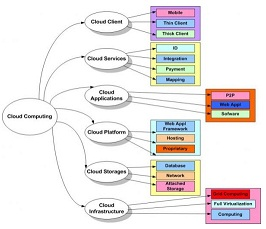
\includegraphics[scale=1]{stiga.jpg} \\
\textbf{Gambar 1.3} Struktur Cloud Computing
\end{center}
\section{Manfaat dan Tujuan Cloud Computing}
\tab Dengan adanya cloud computing akan mengubah paradigma perusahaan ataupun organisasi IT dalam memandang investasi teknologi komunikasi informasi. "Investasi untuk modal kapital berubah menjadi biaya operasional dengan besaran yang lebih efisien akibat adanya cloud computing,dan Ini membuat para pengguna (user) bebas berkreasi dan tidak perlu menyediakan infrastruktur (data center, processing power, storage, sampai ke aplikasi desktop) untuk dapat memiliki sebuah sistem, karena semuanya sudah disediakan secara virtual Disaat ini kebutuhan akan pemakaian , pemeliharaan dan keamanan sistem informasi semakin meningkat, mendorong perusahaan ataupun organisasi untuk meningkatkan dan mengamankan sistem mereka, namun Karena perusahaan ataupun organisasi tidak memiliki sumber daya yang besar untuk membeli sistem untuk keperluan mereka dan bahkan untuk memelihara sistem informasi mereka ,terlebih lagi untuk mengamankan sistem tersebut maka kemungkinan besar Cloud Computing akan menjadi pilihan pertama dan kemungkinan besar akan berkembang, khusunya di Indonesia. Bahkan dengan Cloud Computing, mereka (perusahaan / organisasi) hanya menyewa layanan atau jasa dari penyedia Cloud Computing.
\tab Seperti sudah dijelaskan sebelumnya dengan Cloud Computing ini dapat mengurangi investasi awal dari sebuah perusahaan atau organisasi yang membutuhkan pememakaian, pemeliharaan dan keamanan sistem informasi yanglebih baik. Dalam hal ini investasi yang besar bagi sebuah perusahaan atau organisasi akan berubah menjadi suatu sistem operasional yang mudah dikelola, bahkan penyedia jasa seperti Software as a Service (SaaS) yand ada di Cloud dapat menawarkan harga yang sangat rendah karena faktor ekonomi. Dengan Cloud Computing kita tidak perlu lagi dikuatirkan dengan adanya kompleksitas Teknologi saat ini. Perusahaan dan organisasi yang dalam usahanya menggunakan Teknologi Informasi tidak perlu takut dengan hal-hal yang dapat mengancam keamanan sistem informasi mereka dan bahkan dalam hal peng-updatetan suatu Teknologi atau aplikasi yang dipakai, karena semuanya itu bisa diserahkan kepada penyedia layanan di Cloud Computing. \\Cloud Computing jangan dijadikan sebagai "Core Business" bagi sebuah perusahaan tapi sebaliknya jadikan-lah Cloud Computing ini sebagai "Support Business", prinsip ini yang benar karena Cloud Computing sebagai penunjang suatu perusahaan dalam mengelola sistem informasi yang ada di perusahaan tersebut dengan maksud dan tujuan untuk kelangsungan bisnis dari perusahaan tersebut, karena Cloud Computing memberikan solusi bagi perusahaan untuk meringankan operasional perusahaan tersebut dalam hal pengolahan data. \\Manfaat Cloud Computing :
\begin{itemize}
\item Skalabilitas \\Mudah meningkatkan kapasitas, sebagai kebutuhan komputasi berubah, tanpa membeli peralatan tambahan.
\item Accessibility \\Akses data dan aplikasi melalui internet dari mana saja.
\item Mengurangi Biaya
\item Shift Beban \\Free staf TI internal dari pembaruan dan isu-isu konstan.
\end{itemize}
\tab Keprihatinan utama mengenai cloud computing adalah keamanan dan kehandalan. Banyak organisasi mengalami kesulitan mempercayai informasi mereka dengan vendor pihak ketiga, dan juga penyedia dipublikasikan padam telah meningkatkan keprihatinan mereka. Ketika mengevaluasi kebutuhan komputasi Anda, penting untuk mempertimbangkan baik manfaat dan risiko dari Cloud Computing. Sebagai contoh, data-kerugian yang mungkin baik itu dalam Cloud Computing dan sistem perusahaan tradisional, tetapi dalam banyak kasus vendor Cloud Computing akan memiliki lebih banyak sumber daya yang tersedia dengan cepat dan akurat memperbaiki kegagalan ini. Selain itu dengan teknologi Cloud Computing (komputasi awan) akan memberikan dampak lebih ekonomis dan sumber daya IT yang digunakan lebih efisien, saat aplikasi bisnis dioperasikan dalam suatu lingkungan. Jasa Cloud adalah bisnis yang paling cepat tumbuh dan berkembang pendekatannya untuk memberikan aplikasi dan layanan dari mana saja ke pelanggan apapun, pada perangkat apapun. Sebuah pergeseran yang terjadi dengan komputasi awan yang membentang di alam teknologi dan bisnis, sebuah pergeseran yang dramatis akan mengubah bisnis dan bagaimana menggunakan teknologi untuk memenuhi persyaratan. \\Dengan Cloud Kemampuan untuk menangani tugas-tugas penting, dapat dilakukan
lebih efisien oleh karena dilakukan oleh pihak ketiga, apakah mereka merupakan inti atau bukan inti dengan bisnis anda, adalah sebuah model bisnis yang umum dan merupakan layanan yang bisa menguntungkan anda.
Cloud computing membawa tujuh manfaat potensial, seperti :
\begin{enumerate}
\item Data yang disimpan terpusat.
\item Respon cepat.
\item Kehandalan kode uji.
\item Log (records tak terbetas).
\item Kinerja Perangkat Lunak dengan tingkat keamanan yang tinggi.
\item Konstruksi yang handal.
\item Menghemat Biaya uji keamanan yang mahal.
\end{enumerate}
\tab Selain itu cloud computing dapat memenuhi persyaratan skalabilitas untuk memenuhi permintaan pengguna dengan cepat, namun tidak mengharuskan pengguna untuk menjadi ahli pada bidang teknologi. Dengan teknologi ini kita dapat memfasilitasi workflow application yang berskala besar. Sehingga setiap user yang berorientasi pada penggunaan sistem yang berskala besar untuk keperluan organisasi atau perusahaan-nya, tidak perlu kuatir. Mengapa? teknologi ini (Cloud Computing) hadir untuk mengatasi itu. Sebagai contoh perusahaan yang memerlukan tempat penyimpanan yang besar untuk keperluan kerja perusahaan mereka, cloud dapat menyediakannya, tanpa harus perusahaan tersebut menyediakan server / storage yang besar untuk keperluan data mereka, yang sudah barangtentu memerlukan biaya yang besar. \\Selain itu manfaat dan tujuan dari cloud computing dalam rangka mendukung perangkat lunak yang di gunakan pada Cloud Computing adalah sebagai berikut :
\begin{enumerate}
\item Sistem penagihan yang terencana dan biaya untuk komputasi yang murah pada tingkat yang sangat mantap.
\item Memberikan performance database yang baik dan handal.
\item Memiliki jaminan keamanan yang tinggi yang didukung dengan dedicated server.
\item Memungkinkan pengguna dapat meminta penyimpanan dalam jumlah besar atau kecil dengan cepat serta menyediakan system penyimpanan yang terstruktur yang disebabkan karena ruang penyimpanan yang di atur secara teratur.
\item Mengefisienkan penggunaan aplikasi dan pengefisienan perangkat keras yang selama ini di pergunakan user (semuanya tersedia di Cloud Computing).
\item Menghemat / menekan penggunaan ruang yang berlebihan.
\item Mendukung program go green.
\end{enumerate}
\section{Sejarah Perkembangan Cloud Computing}
\tab Cloud (Awan) adalah suatu istilah yang dipinjam dari telepon. Sampai tahun 1990an, sirkuit data (termasuk yang membawa lalu lintas internet) yang berkabel keras diantara tujuan. Kemudian perusahaan telepon long-haul mulai menawarkan jasa Virtual Private Network (VPN) atau Jaringan Maya Privat untuk komunikasi data. Perusahaan telepon memungkinkan menyediakan layanan yang berdasarkan VPN dengan jaminan bandwidth sebagai sirkuit yang diperbaiki dengan biaya yang lebih murah karena mereka dapat mengganti lalu lintas untuk menyeimbangkan penggunaan yang mereka lihat cocok. Sehingga penggunaan jaringan mereka secara keseluruhan lebih efektif. Sebagai hasil dari penyusunan ini, memungkinkan untuk menentukan dengan cepat dan tepat jalan mana yang akan dilalui. Simbol cloud (Awan) digunakan untuk menunjukkan tanggung jawab sebuah provider (penyedia layanan), dan Cloud Computing (Komputerisasi awan) memperluasnya untuk melindungi server sebaik infrastruktur jaringannya. \\Hal yang mendasari konsep cloud computing berawal pada tahun 1960-an, saat John McCarthy, pakar komputasi MIT yang dikenal juga sebagai salah satu pionir intelejensi buatan, menyampaikan visi bahwa "suatu hari nanti komputasi akan menjadi infrastruktur publik--seperti listrik dan telpon". Namun baru di tahun 1995, Larry Ellison, pendiri Oracle, memunculkan ide "Network Computing" sebagai kampanye untuk menggugat dominasi Microsoft yang saat itu merajai desktop computing dengan Windows 95-nya. Larry Ellison menawarkan ide bahwa sebetulnya user tidak memerlukan berbagai software, mulai dari Sistem Operasi dan berbagai software lain, dijejalkan ke dalamPC desktop mereka. PC Desktop bisa digantikan oleh sebuah terminal yang langsung terhubung dengan sebuah server yang menyediakan environment yang berisi berbagai kebutuhan software yang siap diakses oleh pengguna. Ide "Network Computing" ini sempat menghangat dengan munculnya beberapa pabrikan seperti Sun Microsystem dan Novell Netware yang menawarkan Network Computing client sebagai pengganti desktop. \\Namun akhirnya, gaungNetwork Computingini lenyap dengan sendirinya, terutama disebabkan kualitas jaringan komputer yang saat itu masih belum memadai, sehingga akses NC (Network Computing) ini menjadi sangat lambat, sehingga orang-orang akhirnya kembali memilih kenyamananPC desktop, seiring dengan semakin murahnya harga PC. Merasakan ketidakpraktisan dengan program-program web-based, maka kini diciptakanlah suatu terobosan baru, yaitu Cloud Computing.
\tab Aplikasi yang ada di Cloud Computing tidak tergantung pada sistem operasi yang digunakan oleh pemakai (jadi boleh saja memakai Linux, Mac OS, MS Windows, bahkan sistem operasi PDA atau ponsel). Yang penting, user dapat mengakses Internet, menuju ke alamat atau situs tertentu, untuk menjalankan program yang dia perlukan.Contoh yang paling mudah dijumpai adalah aplikasi Google (di alamat www.google.com/apps) yang di antaranya terdiri atas organiser (pengelola data relasi, jadwal atau kalender, dan email) dan aplikasi bisnis (pengolah kata, pengolah angka, dan program presentasi). Aplikasi tersebut selain gratis, juga selalu diperbarui oleh pembuatnya. Pemakai tidak perlu membayar apapun, kecuali kalau membutuhkan fitur-fitur yang lebih bagus. \\Tonggak selanjutnya adalah kehadiran konsep ASP (Application Service Provider) di akhir era 90-an. Seiring dengan semakin meningkatnya kualitas jaringan komputer, memungkinkan akses aplikasi menjadi lebih cepat. Hal ini ditangkap sebagai peluang oleh sejumlah pemilik data center untuk menawarkan fasilitasnya sebagai tempat hosting aplikasi yang dapat diakses oleh pelanggan melalui jaringan komputer. Dengan demikian pelanggan tidak perlu investasi di perangkat data center. Hanya saja ASP ini masih bersifat "private", di mana layanan hanya dicustomisasi khusus untuk satu pelanggan tertentu, sementara aplikasi yang di sediakan waktu itu umumnya masih bersifat client-server. \\Kehadiran berbagai teknik baru dalam pengembangan perangkat lunak di awal abad 21, terutama di area pemrograman berbasis web disertai peningkatan kapasitas jaringan internet, telah menjadikan situs-situs internet bukan lagi berisi sekedar informasi statik. Tapi sudah mulai mengarah ke aplikasi bisnis yang lebihkompleks. Dan seperti sudah sedikit disinggung sebelumnya, popularitas Cloud Computing semakin menjulang saat di awal 2000-an, Marc Benioff ex VP di Oracle, meluncurkan layanan aplikasi CRM dalam bentuk Software as a Service, Salesforce.com, yang mendapatkan sambutan luar biasa di dunia Teknologi Informasi. Dengan misinya yang terkenal yaitu "The End of Software", Benioff bisa dikatakan berhasil mewujudkan visi bos-nya di Oracle, Larry Elisson, tentang Network Computing menjadi kenyataan satu dekade kemudian. Selanjutnya Cloud Computing bergulir seperti bola salju menyapu dunia teknologi informasi. Dimulai di tahun 2005, mulai muncul inisiatif yang didorong oleh nama-nama besar seperti Amazon.comyang meluncurkan Amazon EC2 (Elastic Compute Cloud), Google dengan Google App Engine-nya, tak ketinggalan raksasa biru IBM meluncurkan Blue Cloud Initiative dan lain sebagainya. 
\tab Semua inisiatif ini masih terus bergerak, dan bentuk Cloud Computing pun masih terus mencari bentuk terbaiknya, baik dari sisi praktis maupun dari sisi akademis. Bahkan dari sisi akademis, jurnal-jurnal yang membahas tentang hal ini baru bermunculan di tiga tahun belakangan. Akhirnya seperti yang kita saksikan sekarang, seluruh nama-nama besar terlibat dalam pertarungan menguasai "awan" ini. Bahkan pabrikan Dell, pernah mencoba mempatenkan istilah "Cloud Computing", namun ditolak oleh otoritas paten Amerika. Walaupun di luaran perebutan ?awan? ini begitu dasyat, tidak demikian dengan di tanah air Indonesia tercinta ini. Pemain yang benar-benar mencoba masuk di area ini masih sangat sedikit, bahkan jumlahnya bisa dibilang belum sebanyak jari sebelah tangan. Salah satu yang cukup serius bermain di area ini adalah PT Telkom, yang setidaknya saat ini sudah menawarkan dua layanan aplikasi berbasis Software as a Service. \\Salah satunya melalui anak usahanya, "Sigma Cipta Caraka", yang menawarkan layanan aplikasi core banking bagi bank kecil-menengah. Kemudian bekerjasama dengan IBM Indonesia dan mitra bisnisnya, PT Codephile, Telkom menawarkan layanan e-Office on Demand untuk kebutuhan kolaborasi/korespondensi di dalam suatu perusahaan atau organisasi. Sepinya sambutan dunia teknologi informasi dalam negeri terhadap Cloud Computing ini, mungkin disebabkan beberapa faktor, di antaranya:
\begin{enumerate}
\item Penetrasi infrastruktur internet yang bisa dibilang masih terbatas.
\item Tingkat kematangan pengguna internet yang masih menjadikan media internet utamanya sebagai media hiburan atau sosialisasi.
\item Tingginya investasi yang dibutuhkan menyediakan layanan cloud ini, karena harus merupakan kombinasi antara infrastruktur jaringan, hardware dan software sekaligus.
\end{enumerate}
\tab Namun demikian, sebagai negara dengan jumlah penduduk terbesar ke-5 di dunia, yang berarti juga pasar terbesar ke-5 di dunia, para pelaku teknologi informasi dalam negeri harus sesegera mungkin mempersiapkan diri dalam arti mulai mengembangkan layanan-layanan yang siap dicloud-kan. Sehingga saat gelombang besar Cloud Computing ini sampai di sini, tidak hanya pemain asing besar saja yang akan menangguk keuntungan. Tentu saja peran pemerintah sebagai fasilitator dan regulator sangat diperlukan di sini. Sampai saat ini paradigm atau pandangan tentang Cloud Computing ini masih berevolusi, dan masih menjadi subyek perdebatan yang melibatkan akademisi, vendor teknologi informasi, badan pemerintah, dan pihak-pihak terkait lainnya. Dan untuk memberikan satu common ground bagi publik, pemerintah Amerika melalui National Institut of Science and Technology (NIST) sebagai bagian dari Departemen Perdagangan Amerika, telah membuat beberapa rekomendasi standar tentang berbagai aspek dari Cloud Computing untuk dijadikan referensi. Beberapa contoh dari sejarah membuktikan bahwa telah berkembang konsep pembuatan kerangka kerja komputasi secara online tersebut - sebagai berikut :
\begin{itemize}
\item Sebuah portal internet yang memiliki berbagai fasilitas layanan umum mulai dari surat elektronik (e-mail), forum diskusi sampai dengan penyimpanan dokumen dengan media penyimpanan yang sangat luas (bahkan ada beberapa yang menyediakan dalam kapasitas tanpa batas/unlimited storage space) - sampai pada mekanisme berbagi dokumen, layananblogdsb. Kesemuanya disediakan dalam sebuah tempat.
\item Layanan Software as a Service atau SaaS dari berbagai vendor teknologi informasi terkemuka - mulai dari layanan pemindaian virus secara online hingga layanan pemindaianspam, dsb.
\item Layanan SpeedyWiki ini secara sederhana dapat dirujuk sebagai dasar-dasar Cloud computing dalam artian fasilitas SpeedyWiki ini dapat diakses dan dipergunakan secara bersamaan untuk berkolaborasi dalam menyusun dokumentasi yang sangat kompleks.
\item Aplikasi Point of Sale atau POS pada kasir pasar swalayan dengan metode Terminal Servicejuga dapat dikategorikan dasar-dasar Cloud Computing.
\end{itemize}
\section{Ragam Penerapan Cloud Computing}
\subsection{Fujitsu terapkan Cloud Computing}
\tab Komputasi awan (cloud computing) saat ini memang sedang marak dilakukan oleh
perusahaan-perusahaan IT, baik lokal maupun internasional. Kini vendor asal Jepang, Fujitsu, yang menerapkannya. perusahaan ini mengumumkan strategi global mereka untuk menerapkan cloud computing yang berlandaskan pada empat model pemakaian sumber daya komputasi, yaitu infrastruktur, aplikasi, aktivitas dan konten. Dalam strategi yang dikembangkan dari pengalaman Fujitsu selama bertahun-tahun, pelanggan bisa menerapkan sebagian atau seluruh model komputasi awan tanpa gangguan. \\Fujitsu telah menawarkan platform ini untuk model infrastruktur yang diperkuat dengan penerapan platform standar komputasi awan global secara luas. Fujitsu Indonesia telah mengembangkan teknologi komputasi awan dengan melihat perubahan dalam masyarakat dan bagaimana teknologi bisa membantu manusia melewati perubahan tersebut. "Inilah yang disebut sebagai sudut pandang human-centric. Di Jepang, Fujitsu berhasil menjalankan uji coba yang melibatkan pertanian dan kesehatan", ujar Achmad S. Sofwan selaku Chief Operation Officer Fujitsu Indonesia. Dimana Uji coba layanan ini sudah dilakukan pada bulan Mei 2010, dilanjutkan dengan komersialisasi pada Oktober 2010 di Jepang, Australia, Singapura, Amerika Serikat, Inggris dan Jerman. Platform komputasi awan global akan menjadi pelengkap platform awan lokal, dengan memenuhi kebutuhan infrastruktur Teknologi Informasi dan Komunikasi (TIK) yang terstandarisasi secara global. Dimana melalui cara ini, diharapkan pelanggan bisa mengadopsi layanan baik dari platform lokal maupun global secara fleksibel. \\Hasilnya, pelanggan bisa mengurangi biaya-biaya TIK, lebih tanggap terhadap kebutuhan bisnis dan bisa menyediakan layanan TIK tanpa mengorbankan keamanan dan tingkat ketersediaan. Pelanggan juga memperoleh manfaat dari keahlian Fujitsu dalam bidang telekomunikasi dan jaringan. Fujitsu sendiri melihat layanan cloud computing sebagi evolusi, bukan revolusi. Untuk itu, model pemakaian sumber daya komputasi di tingkat infrastruktur dan aplikasi adalah perpanjangan dari layanan konvensional yang selama ini ditawarkan Fujitsu. Namun di tingkat aktivitas dan konten, keduanya mencerminkan perubahan signifikan di industri TIK dalam hal menciptakan nilai dengan mengembangkan berbagai model bisnis dan layanan baru bagi para pembeli. \\Berbekal pengalaman selama beberapa dekade dalam menyediakan layanan bisnis, Fujitsu bisa memberikan dukungan kepada pelanggannya untuk berpindah dan bermigrasi ke model komputasi awan secara aman tanpa gangguan. Guna mewujudkan hal ini, perusahaan yang membuka cabang di Indonesia pada 1995 tersebut telah menjalin aliansi dengan sejumlah pihak yang terkait dengan komputasi awan. Mereka menjamin pelanggan tidak akan terjebak dalam sistem-sistem tertutup (proprietary). Berikut kutipan dari Corporate Senior Executive Vice President Fujitsu Richard Christou menyatakan bahwa "Fujitsu akan memberikan layanan komputasi awan terstandarisasi melalui platform cloud global yang digelar secara luas". "Kami akan memberikan pengumuman lanjutan untuk memenuhi fase-fase lain dari model komputasi awan, bersama dengan para mitra kunci di bulan-bulan mendatang. Fujitsu kini dalam posisi untuk bekerja bersama para pelanggan untuk mewujudkan manfaat komputasi awan".
\subsection{Penarapan Cloud Computing pada Google Docs}
\tab Google Docs adalah salah satu produk Google yang dapat mengolah (menyimpan,
membuat, meng-edit) program-program aplikasi perkantoran (seperti microsoft office jika diwindows) secaraonline, diantaranya program-programnya adalah pengolah kata (word processor), pengolah lembar kerja (spreadsheet) dan presentasi (presentation). Penggunakan fasilitas Google DOcs yang harus online/ terkoneksi lewat internet merupakan kelemahan dari program ini, namun aplikasi ini banyak mempunyai kelebihan, misalnya jika kita berpergian keluar kota atau bahkan keluar negeri untuk tujuan seminar atau apa saja kita tidak akan bingung ketinggalan dokumen jika semua sudah disimpan di Google Docs selain itu kita tidak akan kawatir dokumen akan hilang atau rusak seperti halnya jika kita menyimpan di harddisk yang sewaktu-waktu harddisk dapat rusak dan dokumen hilang. Berikut ini adalah hal-hal yang dapat kita lakukan dengan menggunakan Google Docs :
\begin{enumerate}
\item Dalam menggunakan dokumen, yang dapat dilakukan:
\begin{itemize}
\item Upload dokumen Word, OpenOffice, RTF, HTML, atau teks (atau membuat dokumen dari awal).
\item Menggunakan editor WYSIWYG yang sederhana untuk memformat dokumen, memeriksa ejaan, dll.
\item Sharing dengan orang lain (melalui alamat e-mail) untuk mengedit atau melihat dokumen dan spreadsheet.
\item Meng-edit dokumenonlinedengan siapa pun yang kita pilih.
\item Melihat riwayat revisi dokumen dan spreadsheet.
\item Mempublikasikan dokumen secara online ke dunia, sebagai halaman Web atau mengirimkan dokumen keblog.
\item Mendownload dokumen kedesktop sebagai Word, OpenOffice, RTF, PDF, HTML atau zip.
\item Email dokumen sebagai lampiran. \\Dalam menggunakan perangkat lunakspreadsheet, yangdapat dilakukan:
\end{itemize}
\begin{itemize}
\item Mengimpor dan mengekspor data berformat .xls, .csv, .txt dan .ods (dan mengekspor fungsionalitas untuk .pdf dan html).
\item Menikmati navigasi dan pengeditan intuitif, seperti dokumen atau spreadsheet tradisional.
\item Menggunakan format dan formula pengeditan.
\item Mengobrol dengan orang lain yang sedang mengedit.
\item Memasukkan spreadsheet, atau bagian dari spreadsheet, ke blog atau situs web kita. \\Dalam menggunakan perangkat lunak presentasi, yang dapat dilakukan:
\end{itemize}
\begin{itemize}
\item Mengimpor presentasi yang ada dalam jenis file ppt dan .pps.
\item Mengekspor presentasi kita menggunakan fitur Simpan sebagai Zip dari menu File.
\item Mengedit presentasi kita menggunakan editor WYSIWYG yang sederhana.
\item Menyisipkan gambar, dan memformat slide kita agar sesuai dengan keinginankita.
\item Berbagi-pakai dan mengedit presentasi bersama teman dan rekan kerja.
\item Mengizinkan melihat presentasi pada waktu-nyata, online, dari lokasi jauh yang terpisah.
\item Mempublikasikan presentasi kita di web, dan dapat di akses oleh orang lain. \\Untuk besarnya dokumen yang dapat kita kerjakan dalam Google Docs adalah :
\end{itemize}
\end{enumerate}
\begin{enumerate}
\item Dokumen \\
\begin{itemize}
\item Setiap dokumen dapat mencapai sebesar 500K, ditambah 2MB per gambar yang dimasukkan.
\item Dapat meng-upload dokumen dengan format file berikut : \\
\begin{enumerate}
\item HTML
\item Teks biasa (.txt)
\item Microsoft Word(.doc)
\item .rtf
\item Open Office (.odt)
\item Setiap pengguna memiliki batas kombinasi 5000 dokumen dan presentasi serta 5000 gambar.
\end{enumerate}
\end{itemize}
\item Spreadsheet \\
\begin{itemize}
\item Setiapspreadsheet dapat mencapai hingga 10,000 baris, atau hingga 256 kolom, atau hingga 100,000 sel, atau hingga 40 sheet batas mana saja yang tercapai lebih dulu.
\item Setiap pengguna memiliki batas hingga 200 spreadsheet.
\item Batas untuk spreadsheet terbuka pada saat bersamaan adalah 11.
\item Dapat mengimpor spreadsheet hingga mencapai 1 MB dalam format xls, csv, atau ods, txt, tsv, tsb.
\end{itemize}
\item Presentasi \\
\begin{itemize}
\item Setiap presentasi dapat mencapai sebesar 500K, ditambah 2MB per gambar yang dimasukkan.
\item Kita dapat meng-uploadpresentasi dalam format .ppt maupun .pps.
\item Setiap pengguna memiliki batas kombinasi 5000 dokumen dan presentasi serta 5000 gambar
\end{itemize}
\end{enumerate}
\subsection{Penerapan Cloud Computing pada Salesforce.com}
\tab Salesforce.com adalah aplikasi Customer Relationship Management (CRM) berbasis
software as services, dimana kita bisa mengakses aplikasi bisnis: kontak, produk, sales tracking, dashboard, dll. Penerapan Cloud Computing pada Amazon Web Services (AWS) Amazon menawarkan berbagai macam service yang sangat mirip dengan serviceservice yang terdapat pada suatu jaringan konvensional. Membangun jaringan virtual dengan Amazon Web Services sangat mudah dilakukan, namun ada sedikit kesulitan menentukan standar dalam infrastruktur Amzon Web Services, yang disebabkan oleh tidak ada batasan dari penggunaan setiap service yang ada pada Amazon Web Servicies.
\subsection{Penerapan Cloud Computing pada Microsoft Windows Azure (MWA)}
\tab Pada MWA user dimungkinkan untuk mengembangkan aplikasi-aplikasi dengan basis
NET. Dimana user mengembangkan jaringan sesuai dengan kebutuhan, namun MWA menetapkan standar-standar yang tidak bisa dilanggar. Dapat dikatakan atau disimpulkan bahwa MWA merupakan framework-framework aplikasi lengkap yang diimplementasikan dalam jaringan virtual yang memiliki basis yang sama dengan jaringan konvensional.
\subsection{Penerapan Cloud Computing pada Biznet}
\tab Biznet Cloud Computing adalah platform komputer generasi masa depan yang dapat
memberikan keuntungan untuk perusahaan, dimana keuntungannya tetap fokus pada bisnis, tanpa harus memikirkan cara untuk setup, operasi dan menjaga platformkomputer yang berkembang. Platform Biznet Cloud Computing menyediakan pilihan beberapa prosesor, ukuran memory, storage (hard disk) dan berbagai jenis Operating System. Platform ini juga secara otomatis melakukan load balancing sehingga dapat mengirim aplikasi secara maksimal. \\Biznet Cloud Computing menyediakan kemampuan proses komputerisasi dengan standar -standar sebagai berikut :
\begin{itemize}
\item Pilih platform server dan ukuran sesuai kebutuhan
\item Dapat men-setup beberapa server dalam hitungan menit
\item Teknologi virtualisasi berbasis VMware ESXi
\item Akses online melalui control panel danopen API
\item Administration dengan root access
\item Kapasitas Backbone Global Internet Tier-1 secara redundant dengan beberapa Gbps
\item Minimum kontrak 6 bulan
\end{itemize}
\begin{table}
    \begin{tabular}{|c|c|c|}
        \hline
        Layanan                                            & Biaya Bulanan ( Rp ) & Biaya Setup ( Rp ) \\ \hline
        Cloud Server 1 Core, 1 GB RAM, 100 GB SAN Storage  & 2,250,000            & 2,000,000          \\ \hline
        Cloud Server 2 Core, 2 GB RAM, 100 GB SAN Storage  & 3,000,000            & 2,000,000          \\ \hline
        Cloud Server 4 Core, 4 GB RAM, 100 GB SAN Storage  & 4,000,000            & 2,000,000          \\ \hline
        Cloud Server 8 Core, 8 GB RAM, 100 GB SAN Storage  & 5,750,000            & 2,000,000          \\ \hline
        Cloud Server 8 Core, 16 GB RAM, 100 GB SAN Storage & 9,000,000            & 2,000,000          \\ \hline
        Cloud Server 8 Core, 32 GB RAM, 100 GB SAN Storage & 14,500,000           & 2,000,000          \\
        \hline
    \end{tabular}
\end{table}
\tab Seluruh paket Cloud Server termasuk bandwidth inbound \& outbound sebesar 500 GB. Setelah alokasi bulanan telah terpakai, maka ada biaya tambahan sebesar Rp. 2,000/GB untuk tambahan bandwidth yang terpakai. Pada Biznet, pengguna Cloud Computing hanya membayar layanan yang mereka pakai, dimana layanan yang dipakai disesuaikan dengan kebutuhan dari setiap pengguna (user). Sehingga proses pembayaran dilakukan juga sesuai dengan layanan yang mereka pakai (sesuai kebutuhan). Satu virtual Data Center dari layanan Cloud Computing dapat dibagi menjadi beberapa mesin virtual. (kutipan dari Presiden Director Biznet Networks, Adi Kusuma). Cloud Computing adalah teknologi penyimpanan data secara virtual, yang memungkinkan user (pengguna) dapat menyimpan data secara konvensional. \\Melalui Biznet, Cloud Computing yang difokuskan kepada para pengusaha UKM, dimana pengusaha UKM (dalam hal ini sebagai pemilik data) dapat fokus ke bisnis mereka tanpa harus memikirkan biaya yang harus dikeluarkan untuk "membangun" penyimpanan data, karena semua layanan ini dapat disewa dengan mudah, cepat dan yang pasti harga terjangkau. Selain menghemat biaya, Cloud Computing juga mendukung gerakan Green Computing. Ini disebabkan karena layanan Cloud Computing menggunakan server blades yang sangat efisien dalam penggunaan ruang data center dari konsumsi listrik, sehingga dapat mengurangi pemakain listrik yang berlebihan serta polusi lingkungan akibat pembangunan data center yang tidak efisien. Berikut ada beberapa paket yang ditawarkan, antara lain : Cloud Server dengan biaya bulanan Rp. 2,5 juta/bulan, Cloud Hosting Rp. 7 juta/bulan, dan Cloud Storage Rp. 3 juta/bulan.
\section{Riset Cloud Computing}
\tab sumber dari kompas.comdantechno.okezone.com \\
\tab PT Telekomunikasi Indonesia Tbk (Telkom) memperkirakan nilai pasar cloud computing di Indonesia mencapai Rp 2,1 triliun tahun depan. Direktur Whole Sales and Enterprise Telkom Arief Yahya menjelaskan, dari tiga jenis layanan yang bisa diberikan teknologi cloud computing yaitu Software as a Service (SaaS), Platform as a Service (PaaS) dan Infrastructure as a Service (IaaS), maka layanan SaaS paling banyak digunakan. "Dari nilai pasar Rp 2,1 triliun, SaaS menyumbang 40 persen. Kami sendiri akan mengupayakan untuk bisa menguasai pasar sampai 70 persen," kata Arief, Senin (18/10/2010). Arief menambahkan, pasar yang paling banyak menyerap teknologi cloud computing berasal dari instansi pemerintah. Misalnya National Single Windows (NWS), yang berhasil membuat semua pelaku usaha berlomba mendukung program tersebut. \\Hal ini didukung pula oleh belanja IT pemerintah daerah dan pemerintah pusat yang lumayan besar, khususnya untuk pendidikan dan kesehatan. "Di sektor pendidikan saja, ada alokasi Rp 200 triliun, dimana 20 persen untuk belanjaIT". Untuk itu, pemerintah daerah diharapkan tidak segan untuk memanfaatkan cloud computing karena bisa menekan biaya investasi dan menciptakan efisiensi. "Supaya Cloud Computing bisa berkembang, pemerintah harus menerbitkan aturan yang bisa mendorong kerjasama. Mulai dari pemasaran hingga kepemilikan bersama. Di bisnis software saja banyak sekali pemain asingnya. Padahal Cloud Computing modalnya kreativitas. Direktur Utama Teknologi Riset Global Investama (TRG Investama) Gatot Tetuko mengakui, perusahaannya mulai tertarik untuk mencicipi rezeki di bisnis layanan Cloud Computing. "Setelah aktif di penyedian menara dan perangkat Wimax, mereka akan melebarkan sayap ke Cloud Computing karena peluangnya bagus ke depan. TRG Investama adalah pemilik sebagian saham Indonesian Tower dan TRG.
\tab Di bisnis Cloud Computing, TRG Investama akan mengeluarkan merek dagang "Indonesian Cloud". Langkah pertama yang disiapkan oleh perusahaan ini untuk menggarap bisnis cloud computing adalah menggandeng Institut Teknologi Bandung untuk melakukan riset tentang konten-konten spesifik yang terkait dengan Cloud Computing. Dimana TRG Investama menanam Rp 10 miliar untuk melakukan riset hingga jangka waktu tiga tahun mendatang. Cloud computing sama dengan konsep berbagi infrastruktur. Seperti diketahui, selain berpengalaman di bisnis penyediaan menara, Indonesian Tower juga dikenal sebagai penyedia perangkat WiMax. "Ini adalah peluang masa depan yang harus dioptimalkan anak bangsa", tegas Gatot. Menurut dia (Gatot), TRG Investama memiliki keunggulan independen sebagai perusahaan Cloud Computing. \\Pasalnya, posisi independen membuat TRG Investama bebas untuk bekerjasama dengan semua lapisan. Dimana yang menjadi sasaran utama TRG Investama adalah pasar pemerintah dan Usaha Kecil Menegah (UKM). Perlu diketahui,TRG Investama sendiri adalah perusahaan investasi yang memfokuskan diri pada inovasi dan pengembangan teknologi di Indonesia. Dengan dorongan untuk mengembangkan teknologi baru, didukung dengan advance engineering dan manajemen yang berkualitas, TRG Investama bertujuan untuk menciptakan industrial powerhouse di Indonesia melalui anak perusahaannya. Sebelumnya, lembaga riset Gartner memperkirakan dalam waktu dua tahun mendatang sebanyak 80 persen dari perusahaan besar di dunia akan menggunakan Cloud Computing untuk meningkatkan daya saingnya. International Data Corporation memperkirakan tahun lalu pendapatan dari public cloud mencapai 16 miliar dollar AS dan diperkirakan pada 2014 akan mencapai 55,5 miliar dollar AS.
\subsection{Pergerakan Komputasi Awan(Cloud Computing)Semakin Cepat}
\tab sumber dari detik.com \\Sebanyak 83 persen perusahaan berskala besar di Asia Pasifik menilai komputasi awan sebagai teknologi yang relevan bagi bisnis mereka. Persentase ini meningkat lebih dari dua kali lipat dalam 18 bulan terakhir. Demikian hasil survei Springboard Research yang disponsori penyedia solusi virtualisasi VMware. Survei terhadap 6.593 responden pada Bulan September, menunjukkan pergerakan komputasi awan di tujuh pasar Asia Pasifik meningkat pesat selama 18 bulan terakhir ini,khususnya di kalangan perusahaan berukuran besar. Kini, sebanyak 59 persen dari firma regional telah menggunakan atau berencana memakai inisiatif awan (cloud), dibandingkan 45 persen enam bulan lalu dan 22 persen pada 2009. \\Organisasi di Jepang dan Australia memimpin adopsi Awan(cloud), masing-masing dengan 36 persen dan 31 persen telah menjalankan inisiatif yang berkaitan dengan awan(cloud). India dan China adalah yang terdepan dalam hal rencana adopsi, masing-masing 43 persen dan 39 persen tengah berencana menerapkan komputasi Awan(Cloud Computing). Untuk pasar ASEAN, perusahaan di Singapura memimpin dengan 23 persen, disusul Malaysia dan Thailand dengan masing-masing 21 persen. Namun untuk perencanaan awan(cloud), Malaysia dan Thailand adalah yang terdepan masing-masing 29 persen dibandingkan Singapura. Perusahaan-perusahaan yang ahli IT seperti telekomunikasi dan teknologi memimpin baik dalam hal adopsi awan maupun rencana adopsi awan. Perusahaan-perusahaan berukuran besar - terutama yang mempekerjakan lebih dari 10.000 karyawan, memimpin adopsi Awan (39 persen) dibandingkan organisasi yang lebih kecil dengan 100-999 karyawan (20 persen).
\subsection{Teknologi Informasi Berbasis Layanan}
\tab Sebagian besar perusahaan di Jepang (86), Singapura (84) dan Thailand (74)
mengasosiasikan komputasi awan(Cloud Computing) dengan IT-as-a-Service (ItaaS) atau TI sebagai layanan. Di Australia (80), Malaysia (78) dan India (75) mengasosiasikan awan sebagai application-on-demand. Di China, sebanyak 80 responden melihat Awan(cloud) sebagai cara untuk menyediakan storage danjaringan sesuai kebutuhan (on-demand). "Bagi sebagian besar responden survei di Asia Pasifik, TI sebagai layanan adalah tema terbesar hari ini. Perusahaan-perusahaan seperti itu mencari vendor dan konsultan yang mampu membantu mereka menikmati TI berbasis layanan, terutama di area infrastruktur dan manajemen Awan", kata Michael Barnes, VP of Software \& Asia Pacific Research, Springboard Research dalam keterangannya yang dikutip detikINET, Selasa (9/11/2010). Lebih dari separuh organisasi (60) ingin mengadopsi awan(cloud) untuk mencapai skalabilitas sesuai permintaan sehingga bisa lebih cepat memenuhi kebutuhan bisnis, mengurangi biaya infrastruktur peranti keras dan pengadaan server dan sumber daya yang lebih sederhana. Penghematan biaya adalah daya tarik utama dalam mengadopsi komputasi Awan(Cloud Computing), bagi 57 perusahaan di Asia Pasifik. Hanya 37, umumnya perusahaan berukuran besar dengan lebih dari 10.000 karyawan, mengadopsi atau berencana mengadopsi Awan sebagai investasi strategis dalam jangkapanjang.
\subsection{Cloud Computing: Sensasi Masa Depan Dunia IT}
\tab Cloud Computing diperkirakan akan mengubah TI di perusahaan besar karena memungkinkan enterprise dari berbagai ukuran untuk memanfaatkan skala ekonomi dan mendapat keuntungan dari hanya membayar sumber daya yang digunakan saja. Sesungguhnya, banyak aspek komputansi yang sudah (atau akan) tersedia dalam bentuk layanan cloud: Infrastructure as a Service (IAAS) seperti Amazon Services, Microsoft Windows Azure, VMWare vCloud serta Eucalyptus dan Cloudera yang open-source menyediakan komputansi, jaringan serta kapasitas penyimpanan yang elastic. Software as a Service (SAAS) merujuk pada aplikasi online, termasuk software produktivitas, database dan proses bisnis. \\Contoh SAAS termasuk Microsoft Business Productivity Online Suite (BPOS), Google Docs dan Gmail, Salesforce CRM dan Oracle CRM on Demand. Sedangkan, Platform as a Service (PASS), memungkinkan pengembangan aplikasi (contoh, Google Apps dan Windows Azure), Desktop as a Service (DAAS), dan bahkan apa yang disebut sebagai XAAS atauEAAS, yaitu "Everything as a Service". Dengan cloud computing, heterogenitas telah menjadi sebuah karakteristik utama dari komputansi. Sumber daya di awan bisa jadi proprietary atau open-source atau gabungan dari keduanya. Contoh yang menarik bisa dilihat dari profil penawaran dari satu perusahaan berikut ini: Citrix menawarkan aplikasi proprietary seperti GoToMeetings untuk komunikasi desktop dan software konferensi, serta Desktops To Go untuk aplikasi remote desktop. Bersama itu, mereka juga menawarkan produk Open-source seperti server Xen dan XenDesktop, sebuah virtual desktop.
\tab Proyek open-source Xen, yang berada di Citrix, telah melahirkan insiatif bernama Xen Cloud Platform, didukung oleh Citrix, Hewlett-Packard, Intel, Oracle dan Novell. Dengan aplikasinya di Apple iPad, Corix Receiver, Citrix bisa menghadirkan desktop Windows pada iPad, sehingga fungsi desktop dan aplikasi Windows bisa diakses sepenuhnya. Ada tujuh produk Cloud baru, tergabung dalam Citrix Cloud Solutions, yang bersifat open-source dan bisa diperluas sesuai kehendak pengguna. Citrix menyebut Cloud Solutions ini sebagai framework yang memungkinkan interoperabilitas dengan software lain, termasuk virtualisasi pihak ketiga seperti VMWare yang merupakan pesaingnya. Bukan hanya bersifat heterogen karena mencampurkan solusi proprietary dan opensource-- cloud computing juga bersifat global. Sebagai contoh, Windows Azure tersedia di 41 negara. \\Di cloud, pengguna bisa saja mengakses aplikasi yang di-hosting di Hong Kong dari kantornya di Korea Selatan. Datanya, bisa jadi disimpan di server yang ada di Polandia routingnya melalui Amerika Serikat. Dari sudut pandang pengembang piranti lunak, sifat yang global dari cloud ini tak hanya ditentukan oleh perilaku jejaringnya, tapi juga struktur bisnis itu sendiri. Peneliti yang bekerja untuk perusahaan multinasional asal AS di Russia mungkin berkolaborasi dengan tim di Singapura. Produk akhirnya bisa jadi dirancang di AS dan Taiwan, dibuat di India, Malaysia, dan Filipina untuk dijual di Amerika Selatan. Peluang ekonomi ada bagi negara yang memiliki kebijakan publik dan hukum yang netral secara teknologi dan kompatibel. Contohnya, pemerintah Singapura yang sejak lama menyadari bahwa teknologi mendorong pertumbuhan ekonomi negara itu. Di 2008, pemerintahannya bekerjasama dengan Hewlett Packard, Intel dan Yahoo, serta lembaga penelitian di Russia, Jerman dan AS untuk membuat test bed open-source yang mendukung penelitian layanan cloud pada skala global. HP juga membuka Cloud Labs di Singapura. Di saat yang sama, pemerintahannya memberi subsidi pada proyek yang bisa memberikan Cloud Computing pada eGovernment dan Usaha Kecil Menengah. Singapura adalah pemimpin dalam melihat Cloud Computing sebagai alat menumbuhkan ekonomi IT-nya serta menjaga perannya di pasar global. Memang masih di tahap awal, tapi jelas bahwa ini akan mengubah komputansi di enterprise, memenuhi kebutuhan pengguna dengan kelenturan yang belum pernah dilihat sebelumnya. \\Dengan makin tumbuhnya Cloud Computing, maka semakin penting bagi pembuat kebijakan untuk menjamin bahwa kebijakan domestiknya tidak berpihak pada teknologi tertentu. Bukan hanya untuk memenuhi kebutuhan perdagangan global, hukum internasional dan kepentingan pertumbuhan ekonomi, hal ini juga memungkinkan perusahaan domestik untuk meraup keuntungan besar dari peluang yang dihasilkan cloud computing.
\subsection{Membangun Infrastruktur Cloud Computing Masa Depan}
\tab sumber : CHIP.co.id \\Cloud Computing membawa perubahan mendasar pada cara orang dan berbisnis menggunakan internet serta perangkat komputasi. Tercatat 175 exabyte data melintasi internet pada tahun 2010, setara dengan 43.750 juta DVD. Dengan kondisi seperti ini, evolusi Cloud Computingyang mengandung arti lebih banyak pengguna, lebih banyak perangkat, konten lebih kompleks dan harapan yang lebih besar di mana saja, kapan saja untuk mengakses data. Cloud Computing menjadi sebuah kenyataan di Asia Pasifik dan industri telah mulai berpikir tentang bagaimana hal ini akan menguntungkan dan memajukan bisnisdi masa akan datang. Jason Fedder, General Manager, Asia Pasific \& Cina, Data Center Products Group,
Intel, mengundang CHIP.co.id bergabung dalam telekonferensi dengan wartawan dari berbagai negara di Asia Pasific dan Cina dalam sebuah diskusi tentang masa depan Cloud Computing. Pada telekonferensi kali ini dibicarakan teknologi yang dibutuhkan untuk mendukung Cloud Computing dan kemitraan di masa depan. Intel membagikan visi pada CHIP.co.id tentang Cloud Computing di Tahun 2015, dan menjelaskan beberapa gagasan dan istilah, tentang Cloud yaitu Federated, Automated, Client Aware.
\begin{enumerate}
\item Federated berarti sejumlah data yang ada pada berbagai perangkat dapat dipertukarkan secara aman melalui Cloud, baik lintas publik maupun private.
\item Automated berarti Pertukaran data tersebut juga dapat berjalan sendiri secara otomatis sehingga di masa depan, berbagai pihak dapat lebih fokus pada inovasi dan berkurang dari sisi manajemen data.
\item Client Aware berarti, layanan bisa dioptimasi, ditingkatkan sesuai dasar kemampuan perangkat yang ada.
\end{enumerate}
\tab Selain tiga hal ini Jason Fedder juga membahas Open Data Center Alliance di mana lebih dari 70 bisnis global disatukan oleh Intel untuk membuat panduan untuk interoperabilitas, fleksibilitas dan standar industri untuk Cloud Computing. Open Data Center Alliance ini telah diluncurkan sejak 27 Oktober 2010. Intel juga membentuk Intel ® Cloud Builders, sebuah kemitraan 20 hardware terkemuka di dunia dan pembuat perangkat lunak yang akan menjadi referensi serta mengikat sumber daya untuk mendorong inovasi dan membuat teknologi Cloud Computingmudah untuk disebarkan, digunakan dan berbagi pengetahuan. Yang menjadi pertanyaan bagaimana dengan perkembangan Teknologi Cloud Computing untuk masa yang akan datang di Indonesia? "Cloud computing tidak bisa dihindari, dengan menggunakan layanan tersebut para pelaku industri akan lebih meningkatkan efisiensi perusahaannya, terutama untuk kelas UKM (usaha kecil menengah)", jelas Philip Sargeant, Research VP Gartner kepada sejumlah wartawan, seperti yangdilansir oleh laman detikcom. \\Menurut data Gartner, di tahun 2010 ini diperkirakan nilai bisnis dari pemanfaatan teknologi internet untuk menyediakan sumber komputer itu sendiri secara global mencapai USD 80 miliar dengan tingkat pertumbuhannya setiap tahun sebesar 25 persen dalam jangka waktu lima tahun mendatang. Jadi, bisnis ini akan menjadi bisnis yang akan semakin ramai seiring dengan murahnya harga bandwidth. Semua tergantung kebutuhan, jika data bersifat tidak confidential saat ini pun bisa dimulai. Sebaliknya jika memerlukan sistem keamanan yang baik, maka akan bisa dimulai beberapa tahun kedepan, tergantung dari layanan yang dibutuhkan.